\chapter{Algorithms}

\section{Grammar with disambiguation list for Disambiguation: GELD}

	The problem with the new kind of grammar, compared to the old SLG is that we
	have ambiguity in it. For example: \\
	\begin{center}
	$S \rightarrow \textbf{N}gaacca\textbf{N}tggaccg$\\
	$N \rightarrow u I v$ \\
	$I \rightarrow y_1 | y_2$
	\end{center}

	When decoding, each time an N appears we don't know if we have to replace the inside
	I with and $y_1$ or a $y_2$

	Hence, we have to add some information to avoid this issue. That could be and
	disambiguation list telling us what inside should be used. But this introduce a penalty
	in the grammar size in each iteration k: \\
	\begin{center}
		$|G_k| + |Encoding_k|$
	\end{center} 

	So, in this approach we should add to the score function the size of the disambiguation list
	in each iteration. \\

	The list can be represented in many different ways. For example, 
	\begin{itemize}
		\item for each non terminal we could have a queue with the elections of the 
		insides of the non terminal. When we decode, each time we see this non terminal appear
		we pop the next element from the queue and see which option should be used: \\


	$S \rightarrow \textbf{N}gaacca\textbf{N}tggaccg$\\
	$N \rightarrow u I v$ \\
	$I \rightarrow y_1 | y_2$  encoding queue: [1, 2] \\

	In this approach we are already compressing the disambiguation list, because we don't
	need to add an encoding element for each election. \\
	For example, if we have the next rule:\\

	$S \rightarrow \bm{N_2}gaacca\textbf{N}tggaccg\textbf{N}\textbf{N}aggtg\textbf{N}$\\
	$N \rightarrow \bm{N_2} agt$ \\
	$N_2 \rightarrow uIv$\\
	$I \rightarrow y_1 | y_2$  encoding queue: [1, 2]

	doesn't matter how many times we have the N non terminal, because we always know
	that the $N_2$ inside it has always the encoding 2.


		\item A sequence ordered in preorder, postorder, inorder, etc. based on the parse
		tree generated by the grammar. \\

		By ordering the sequence, we could also get intereseting structural motifs. But
		we need an encoding element for each time a non terminal with elections appears
		in the parse tree. \\

		reusing our last example: \\

		$S \rightarrow \bm{N_2}gaacca\textbf{N}tggaccg\textbf{N}\textbf{N}aggtg\textbf{N}$\\
		$N \rightarrow \bm{N_2} agt$ \\
		$N_2 \rightarrow uIv$\\
		$I \rightarrow y_1 | y_2$  encoding queue: [1, 2, 2, 2, 2]

	\end{itemize}



	\subsection{Pseudocode}

	\begin{algorithm}
	\caption{GELD}
	\begin{algorithmic}[1]
	\REQUIRE Sequence S
	\WHILE{Grammar size can improve}
	\STATE bestYield = getBestYieldBasedOnScore(allPossibleYields(S))
	\STATE replaceYield(S, bestYield)
	\STATE addProductionToSequence(N, bestYield) 
	\STATE N++
	\ENDWHILE

	\end{algorithmic}
	\end{algorithm}


	\begin{algorithm}
	\caption{replaceYield}
	\begin{algorithmic}[1]
	\REQUIRE Sequence S, yield
	\STATE yieldPos = getYieldPositions(S, yield)
	\FOR{pos in yieldPos}
		\STATE i = currentInside(pos)
		\STATE replace yield by $N$
		\STATE encodingList.insert(i) 
	\ENDFOR
	\end{algorithmic}
	\end{algorithm}




	\subsection{Compressing disambiguation list}

	If we manage to	construct the disambiguation list in a way that is structurally interesting we could
	compress it effectively. \\

	Efforts have been made to do it in a Depth-first search (DFS) approach. \emph{DFS is an algorithm for traversing or searching tree or graph data structures. One starts at the root (selecting some arbitrary node as the root in the case of a graph) and explores as far as possible along each branch before backtracking.}
	(\url{http://en.wikipedia.org/wiki/Depth-first_search}) \\

	Complications were found during the implementation and DFS couldn't be done directly from the desambiguation
 list, but from a parse tree. Building Parse Trees is big time and resource consuming. In future work this will be a priority. \\

	There are some ways not to add this type of penalties as a list outside the grammar,
	but inside it as new symbols. This approach will be explained in the next section. \\

	\newpage

	\section{Straight Line Inplace Disambiguation (SLID)}

	Instead of adding the same non terminal N to replace each yield in each iteration,
	 and an disambiguation list to remember
	the inside selection, we can use a new symbol $(N_{+i})$ to refer
	to the inside $Y_i$ inside the $N$ rule. By doing so, we don't need an encoding
	scheme outside the grammar, because the information remains implicit in the new symbol. 
	The counterpart	is that we are adding new symbols and this affect as the iterations
	increase. \\

	Our grammar would be like this: \\
	\begin{center}
	$S \rightarrow \bm{N_{+1}}gaacca\bm{N_{+2}}tggaccg$\\
	$N \rightarrow u I v$ \\
	$I \rightarrow Y_1 | Y_2$
	\end{center}

	The decode is straightfoward rightnow, because we construct the grammar and
	do the replacements in such a way that there's no possible ambiguity. Now we have
	a symbol for each inside used. So, if we have for example $N_{+1}$ we know we are 
	refering to inside $Y_1$.\\

	The SLID approach is extremelly useful in small sequences that doesn't need so many
	iterations. When the sequence get bigger, we reduce in each iteration the possibility
	of compressing by adding new symbols. \\


	\subsection{Pseudocode}

	\begin{algorithm}
	\caption{SLID}
	\begin{algorithmic}[1]
	\REQUIRE Sequence S
	\WHILE{Grammar size can improve}
	\STATE bestYield = getBestYieldBasedOnScore(allPossibleYields(S))
	\STATE replaceYield(S, bestYield)
	\STATE addProductionToSequence(N)
	\STATE N += numberOfDifferentInsides(N)
	\ENDWHILE

	\end{algorithmic}
	\end{algorithm}


	\begin{algorithm}
	\caption{replaceYield}
	\begin{algorithmic}[1]
	\REQUIRE Sequence S, yield
	\STATE yieldPos = getYieldPositions(S, yield)
	\FOR{pos in yieldPos}
		\STATE i = currentInside(pos)
		\STATE replace yield by $N_{+i}$ 
	\ENDFOR
	\end{algorithmic}
	\end{algorithm}

	\newpage

	\section{Parse Tree + SLID (PT+SLID)}

	To avoid adding new symbols in each iteration, we said one thing we can do is
	to have the disambiguation list outside the grammar. In each iteration we replace by just an $N$ as in $GELD$
	instead of $N_{+1}$, $N_{+2}$ as in $SLID$. 

	At the end, based on the encoding, we can parse the grammar and traverse the tree
	generated. 

	By traversing it in a preorder manner, we add new Non Terminals to differenciate 
	the N that we didn't differenciate before.  It means, that if we have to subtrees
	with the same root but different nodes inside it, we separate it in as many rules
	as differences we have.\\

	\emph{A preordering is a list of the vertices in the order that they were first visited by the depth-first search algorithm. This is a compact and natural way of describing the progress of the search} (\url{http://en.wikipedia.org/wiki/Depth-first_search}).\\

	Basically, we follow $GELD$ and when we reach the final grammar we convert it 
	to a $SLID$ grammar.

	In the next section	this concept will be clarified.

	\newpage


	\subsection{Algorithm}

	Starting from the result of GELD, a grammar and and its disambiguation list, we want to obtain
	a grammar with the encoding implicit in it, as in the SLID approach. \\

	We must use a different heuristic score for each iteration, because we are not having
	an disambiguation list at the end. Until now we are using the same score but without
	the encoding penalty. \\

	We can think the algorithm as traversing a Parse Tree generated by the grammar and changing/adding some new non terminals on the fly. \\

	We start in the root of Parse Tree and traverse the tree in a preorder way. \\

	% We have two different possibilities: \\
	% \begin{itemize}
	% 	\item[1] Non Terminal whose children are all \emph{terminals} (could be already visited Non Terminals).
	% 	\begin{center}
	% 				\includegraphics{images/PT+SLID1option.png}
	% 	\end{center}
	% 	\item[2] Non Terminal whose children has at least one Non Terminal
	% 	\begin{center}
	% 				\includegraphics{images/PT+SLID2option.png}
	% 	\end{center}
	% \end{itemize}

	% The first option is straightfoward: we just add that non terminal with its children as a Production in the final grammar.\\

	% The second case is trickier. We have to enter recursively in each of its non terminals to obtain to numbers who will identify the analysed non terminal: $i$ and $j$ \\

	For each Non Terminal N node we reach, we add it with his children
	as a production to a productions set $P$. \\

	If this non Terminal was an Inside, we assign a $j$ value based on the option we
	are adding. \\

	$j$: is refered to the inside election of the current non terminal.
	For example:\\
	$M_{+j}$ means that we are in the $j$ option from the inside $I$ of $M$ in our parse tree traversing. \\

	Now, each non terminal $N$, must be separated in $N_1$, ..., $N_n$, based on 
	the $M_{+j}$ inside them. \\

		For example, watching the parse tree, we got that N could be:\\

	$N \rightarrow M_{+\textbf{1}} agt I$\\

	But in another subtree it could be: \\

	$N \rightarrow M_{+\textbf{2}} agt I$ \\

	so we separate these two cases in: \\

	$N^\textbf{1} \rightarrow M_{+\textbf{1}} agt I$\\

	$N^\textbf{2} \rightarrow M_{+\textbf{2}} agt I$ \\

	So we need to add the index i to make a distinction within them: $N^i$\\


	$N^i_{+j}$ means that, we choose the N non terminal with index $i$ and with option
	$j$ in its \emph{Inside}.\\

	\newpage

	Example of the resulting grammar: \\

	Original $S = gtggaccgaccacagagacctgaccgttggaacgaccacagaagaacacca$\\

	$S \rightarrow g - 10^1 - 8_{+1} - t - 8_{+1} - g - t - 10^2_{+1} - a - 8_{+2} - a - c - c - a$ \\

	$7 \rightarrow c | a$\\

	$8 \rightarrow g - a - 7 - c$ \\

 	$9^1 \rightarrow 8_{+1} - a - c$ \\

	$10^1 \rightarrow t - g - 8_{+1} - 9^1 - a - g - a$ \\

	$10^2 \rightarrow t - g - 8_{+2} - 9^1 - a - g - a$\\


	With all these new symbols added, there's no ambiguity, so we can just follow
	the non terminals and unfold them. \\ 

	The resulting grammar will be different to the original SLID version, because
	in each iteration we weren't adding new symbols that decrease drastically our
	compression power. \\



	\newpage

	\subsection{Pseudocode}

	\begin{algorithm}
	\caption{PT+SLID}
	\begin{algorithmic}[1]
	\REQUIRE Grammar G
	\STATE Run GELD algorithm with modify score
	\STATE Build Parse Tree PT from G based on disambiguation list
	\STATE prods = map\{int, list\} \COMMENT{the list will save the different right sizes (rhs) of N}
	\STATE preNodeList = getNodesInPreorder(PT)

	\FOR{N in preNodeList}
		\STATE rhs = N.rhs()
		\IF{N not in prods}
			\STATE prods.insert(N, rhs)
		\ENDIF
		\IF{N in prods but with a different rhs}
			\STATE prods(N).append(rhs)
			\STATE i = rhsPosInProds(N)
		\ENDIF
		\IF{lastInside is N's inside}
			\STATE Modify N adding j in parse tree: $N_{+j}$
			\STATE update preNodeList
		\ENDIF

		\IF{isInside(N)}
			\STATE lastInside = N
			\STATE j = i
		\ENDIF

	\ENDFOR	

	\end{algorithmic}
	\end{algorithm}

	\subsection{Possible Problems with PT+SLID approach}

	\begin{itemize}
		\item The problem here is that we have to generate a parse tree, or an implicit 
	parse tree, carrying implementation difficulties and performance problems (
	memory consumption with large corpus).

		\item The problem is that the final grammar has many similar rules, so we should find
	a way to factorize the rules to avoid this problem.\\

	For example: 

	$10^1 \rightarrow t - g - 8_{+1} - 9^1 - a - g - a$ \\

	$10^2 \rightarrow t - g - 8_{+2} - 9^1 - a - g - a$\\

	could be written as:

	$10^1 \rightarrow t - g - 8_{+1}, 8_{+2} - 9^1 - a - g - a$ \\

	or something similar.

		This carries again implementation issues.
		
	\end{itemize}



	% \begin{algorithm}
	% \caption{PT+SLID}
	% \begin{algorithmic}[1]
	% \REQUIRE Grammar G and Encoding $E_g$

	% 	\COMMENT{Base case:}
	% \STATE Check if current non terminal N already exists in $G_f$

	% \IF{exists(N)}
	% 	\STATE add new Production N with index i+1 (where i was the last pos of the last N)
	% \ENDIF
	% \IF{!exists(N)}
	% 	\STATE add Production N to $G_f$
	% \ENDIF
	% \STATE Mark N as visited

	% \COMMENT{Recursive case:}
	% \WHILE{there's a children from N, named c}
	% 	\IF{isNonTerminal(c) and !visited(c)}
	% 		\STATE j = PT+SLID(c) \COMMENT{Recursive call, j is the I option number, assign only if c = I}
	% 	\ENDIF
	% 	\IF{!isNonTerminal(c)}
	% 		\STATE append c to N production
	% 	\ENDIF
	% \ENDWHILE

	% \STATE Repeat similar to base case to check existance, and to obtain $i$. 
	% \STATE Add $N^i + j$ to productions if it didn't exist. 
	% \STATE Mark $N^i + j$ as visited.

	% \end{algorithmic}
	% \end{algorithm}



		% ENCODING TREE:
		% As we can see, we have and 8 Non Terminal inside de 10 rule. So we can build
		% a tree in the following way, to include all possible ways to unfold the non
		% terminal 10: \\

		% 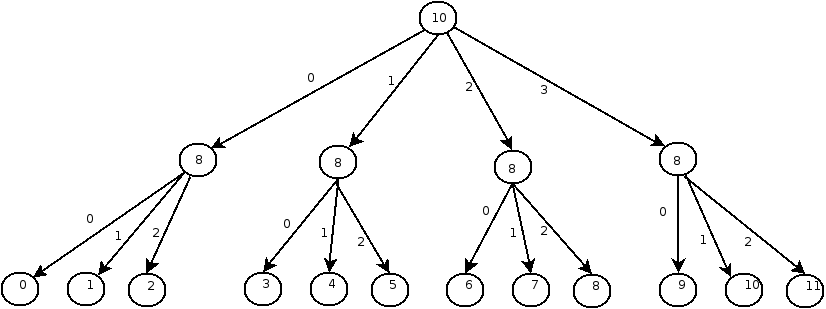
\includegraphics[scale=0.5]{images/DecodeTree.png}

		% Each leaf is a possible completely unfolded replacement.
		% In our example, the first apparition of non terminal 10 has the encoding 2,
		% and our first 8 the encode 1, so we have to follow the path 2-1 in our tree,
		% ending in the leaf number 7.

		% As a result, we have to replace our non terminal 10 with a 10+7 non terminal:

		% \begin{center}
		% \begin{flushleft}
		% $S \rightarrow ----17---10----10----10---8$ \\
		% $7 \rightarrow ---|---$ \\
		% $8 \rightarrow u7v$, encoding: 1, 2, 1, 1, 0\\
		% $9 \rightarrow --- | --- | ---$ \\
		% $10 \rightarrow ---9 ---8 --$, encoding: 2, 3, 1, 0 \\
		% \end{flushleft}
		% \end{center}

		% In the same way we replace every single highest Non Terminal. As a final result
		% we've got the follow gramamr:

		% \begin{center}
		% \begin{flushleft}
		% $S \rightarrow ----17---21----14----11---8$ \\
		% $7 \rightarrow ---|---$ \\
		% $8 \rightarrow u7v$\\
		% $9 \rightarrow --- | --- | ---$ \\
		% $10 \rightarrow ---9 ---8 --$\\
		% \end{flushleft}
		% \end{center}

		% And we can unfold it, just by rebuilding the trees based on the new symbols. \\
		% For example, taking the 17, we know it correspond to the non terminal 10. We
		% get inside the 10 rule and watch that the 9 has 3 possibilities, so we build
		% 4 branches in the tree (3 possibilities plus the epsilon). After that, we
		% continue and an 8 appears. We enter in the 8 rule and watch that is has 2 possibilites,
		% so we add 3 branches from each leaf of the last step. The we just search for
		% the leaf that gives us the 17.


		% The problem is that the tree gets really big:\\
		% $size(Tree(N)) = \prod_{N_i \in N} size(Tree(N_i))$\\

		% Is like using a pairing encoding function.
